%
% main.tex -- Paper zum Thema <maxwell>
%
% (c) 2020 Autor, OST Ostschweizer Fachhochschule
%
% !TEX root = ../../buch.tex
% !TEX encoding = UTF-8
%

\chapter{Maxwell\label{chapter:maxwell}}
\kopflinks{Maxwell}
\begin{refsection}
\chapterauthor{Maurin Doswald und Stephan Oseghale}

Als James Clerk Maxwell 1865 seine Arbeit über das elektromagnetische Feld veröffentlichte, gelang ihm das Wesen des elektrischen- und magnetischen Feldes, sowie die Interaktion jener mathematisch zu beschreiben und somit das Grundwesen der Elektrodynamik aufzuzeigen.
Durch seine theoretische Arbeit konnte die Existenz von elektromagnetischen Wellen und dass sich diese mit Lichtgeschwindigkeit ausbreiten experimentell Nachgewiesen werden.
Dies führte zu Technologien wie Radio, Radar, Fernseher und viele weitere Anwendungen in der drahtlosen Kommunikation.

Die Grundidee zur Formulierung dieser Gleichungen kam durch eine Reihe von experimentellen Beobachtungen und theoretischen Ansätzen unterschiedlichster Wissenschaftler unter anderem Michael Faraday und André-Marie Ampère.
Durch mathematische Analysen und Experimente entwickelte Maxwell schlussendlich 20 Gleichungen, welche später von Oliver Heavyside und Willard Gibbs in die heutige bekannte vektorielle Schreibweise von vier Gleichungen gebracht wurden.
Das Ziel dieser Arbeit ist aufzuzeigen, dass die vier fundamentalen Gleichungen sowohl auch über ein Variationsprinzip hergeleitet werden können.

%
% mathFormulierung.tex -- Felder und deren Operationen
%
% 
%
% !TEX root = ../../buch.tex
% !TEX encoding = UTF-8
%
\section{Felder\label{maxwell:mathFormulierung}}
\rhead{Felder}

Da sowohl das elektrische Feld $\vec{E}$ wie auch das magnetische Feld $\vec{B}$ als Vektorfeld beschrieben werden, soll hier der Begriff des Feldes erläutert und grafisch aufgezeigt werden.

\subsection{Skalarfeld\label{maxwell:skalarfeld}}

Ein Skalarfeld ist eine Funktion der Form
\[ f:\mathbb{R}^n \rightarrow \mathbb{R}, \] 
die jedem Punkt im Raum ein Skalar zuordnet.
Alltägliches Beispiele für ein Skalarfelder sind Temperaturverteilungen, Ladungsdichten oder Potentiale. In \ref{maxwell:skalarGrad} ist der Querschnitt eines Skalarfeldes abgebildet.


%Zu den wichtigsten Operationen eines Skalarfeldes gehört der Gradient, welcher dem Skalar- ein Vektorfeld zuordnet.
%Sei $\phi$ ein Skalarfeld, dann ist $\nabla\phi$ ein Vektorfeld, dargestellt in \ref{maxwell:skalarGrad}.

\begin{figure}
	\centering
	\subfigure{\includegraphics[width=0.35\textwidth]{papers/maxwell/skalar}}
	\subfigure{\includegraphics[width=0.3\textwidth]{papers/maxwell/gradient}}
	\caption{Skalar- und Vektorfeld}
	\label{maxwell:skalarGrad}
\end{figure}

\subsection{Vektorfeld\label{maxwell:vektorfeld}}

Ein Vektorfeld ist eine Funktion der Form \[ f: \mathbb{R}^n \rightarrow \mathbb{R}^m, \] welche jedem Punkt im Raum einen Vektor zuweist. 
Die Richtung dieses Vektors gibt hierbei an, in welche Richtung der Fluss des Feldes an diesem Punkt geht, während der Betrag die Intensität repräsentiert.


Des weiteren spricht man von stationären Vektorfelder, wenn sie zeitunabhängig sind und von homogenen Vektorfelder, wenn die Richtung und der Betrag der Vektoren ortsunabhängig sind, also wenn jeder Vektor die gleiche Richtung und den gleichen Betrag haben. 
Wie bereits erwähnt, sind das elektrische und das magnetische Feld, wie auch andere Kraftfelder Beispiele von Vektorfelder.
Der Querschnitt eines Vektorfeldes ist auch in \ref{maxwell:skalarGrad} abgebildet.

\subsection{Operationen}

\subsubsection{Gradient}

Der Gradient wurde bereits in \ref{buch:fuvar:richtungsableitung:def:gradient} definiert, dieser Operator, welcher auf ein Skalarfeld angewendet wird, resultiert in einem Vektorfeld. 
Die Richtung der Vektoren dieses neuen Vektorfeldes zeigen demnach immer in die Richtung der grössten Zunahme.
%Weiter unten wird ersichtlich, dass auch das elektrische Feld ein Gradientenfeld ist \[ \vec{E} = -\nabla\varphi, \] wobei $\varphi$ das elektrische Potential ist.

\subsubsection{Divergenz}
%TODO: Link auf Kapitel von Müller
Die Divergenz eines Vektorfeldes $\vec{F}$ ist definiert als 
\[ \nabla\cdot\vec{F}. \]
Angewendet wird sie auf ein Vektorfeld und resultiert in ein Skalarfeld.
Die Divergenz sagt aus, ob an einem Punkt mehr ``hinein-'' als ``rausfliesst'' und macht so eine Aussage über das Bestehen von Quellen und Senken.

Wenn die Divergenz negativ ist, liegt eine Senke vor, wenn sie positiv ist eine Quelle.
Ein Vektorfeld wird quellenfrei genannt, wenn seine Divergenz zu null resultiert.

\subsubsection{Rotation}
%TODO: Link auf Kapitel von Müller
Die Rotation eines Vektorfeldes $\vec{F}$ ist definiert als,
\[ \nabla\times\vec{F}. \]
Mit dieser Operation wird einem Vektorfeld ein neues Vektorfeld zugeordnet, welches eine Aussage macht, wie stark das Feld sich um einen Punkt dreht bzw. rotiert.
Wenn die Rotation zu null resultiert, ist das Feld wirbelfrei.

%
% einleitung.tex -- Beispiel-File für die Einleitung
%
% (c) 2020 Prof Dr Andreas Müller, Hochschule Rapperswil
%
% !TEX root = ../../buch.tex
% !TEX encoding = UTF-8
%
% erste Maxwellgleichung ohne Quelle

\tikzset{>=latex} % for LaTeX arrow head
\usetikzlibrary {arrows.meta}
\pgfplotsset{compat=1.13}
\usetikzlibrary{decorations.markings,intersections,calc}
\usetikzlibrary{angles,quotes} % for pic (angle labels)
\colorlet{Ecol}{green!90!black}
\colorlet{EcolFL}{green!80!black}
\colorlet{Bcol}{blue!90!black}
\tikzstyle{EcolEP}=[blue!80!white]
\colorlet{veccol}{green!45!black}
\tikzstyle{charge+}=[very thin,top color=red!50,bottom color=red!90!black,shading angle=20]
\tikzstyle{charge-}=[very thin,top color=blue!50,bottom color=blue!80,shading angle=20]
\tikzstyle{charge_small} = [very thin,top color=red!50,bottom color=red!90,shading angle=20]
\tikzstyle{vector}=[->,thick,veccol]
\tikzset{EFieldLineArrow/.style={EcolFL,decoration={markings,mark=at position #1 with {\arrow{latex}}},
		postaction={decorate}},
	EFieldLineArrow/.default=0.5}


\section{Elektrostatik\label{maxwell:section:elekktrostatik}}
\rhead{Elektrostatik}
Die Elektrostatik ist ein Spezialfall der Elektrodynamik, bei dem statische Felder betrachtet werden.
Dies setzt voraus, dass
\begin{equation}
	\frac{\partial f}{\partial t}
	=
	0
	\qquad
	\forall f,t.
	\label{maxwell:section:definition_statik}
\end{equation}
Daraus folgt, dass wir nur ruhende Ladungen betrachten.
Dies hat zur Folge, dass keine Stromdichten existieren können, weil
\begin{equation}
	\rho(x,y,z) \underbrace{\vec{v}}_{=0}
	=
	\vec{j}(x,y,z)
	=
	0.
\end{equation}
Im späteren Abschnitt \ref{maxwell:magnetostatik} der Magnetostatik wird klar, dass aus diesem Grund in der Elektrostatik keine magnetische Flussdichte existieren kann.
 
Das Ziel ist nun das elektrische Feld im Zusammenspiel mit ruhenden Ladungen zu beschreiben.
Dafür werden wir in den folgenden Abschnitten die nötigen Begriffe definieren und genauer erklären.

%TODO: Ladung noch definieren? (denke nicht)
\subsubsection{Elektrisches Potentialfeld}
Das elektrische Potentialfeld
\[
\phi:\mathbb{R}^3
\rightarrow
\mathbb{R}
\]
ist als
\begin{equation}
	\phi(x,y,z)
	=
	\frac{W_{pot}(x,y,z)}{q}
	\label{maxwell:section:definition_elektrischespotentialfeld}
\end{equation}
definiert.
In Worten gefasst kann man sagen, dass das elektrische Potential eine auf Ladung normierte, potentielle Energie darstellt.
Somit kann die linke Abbildung in \ref{maxwell:skalarGrad} als ein Feld, das proportional zur potentiellen Energie ist, angeschaut werden.
Des Weiteren steht die elektrische Spannung eng in Verbindung mit dem elektrischen Potential.
Die Spannung $U$ zwischen zwei Punkten $a$ und $b$ wird definiert als
\[
U_{ab}
=
\phi_a - \phi_b.
\]
% not sure about this
Das heisst die Spannung ist der Potentialunterschied zwischen zwei Punkten.

\subsubsection{Elektrisches Feld}
Das elektrische Feld
\[
\vec{E}:\mathbb{R}^3 \rightarrow \mathbb{R}^3
\]
wird ganz allgemein definiert als
\begin{equation}
\vec{E}(x,y,z)
=
- \nabla\phi(x,y,z) - \frac{\partial \vec{A}}{\partial t}(x,y,z),
\label{maxwell:section:definiton_allgemein_elektrischesFeld}
\end{equation}
wobei $\vec{A}$ das magnetische Vektorpotential ist \eqref{maxwell:definitionVektorpot}.
Da wir dank Gleichung \eqref{maxwell:section:definition_statik} wissen, dass alle zeitlichen Ableitungen null sein müssen, ist die statische Definition des elektrischen Feldes
\begin{equation}
\vec{E}(x,y,z)
=
- \nabla\phi(x,y,z).
\label{maxwell:section:definition_statisch_elektrischesFeld}
\end{equation}
Diese Definition besagt, dass das elektrische Feld ein statisches Gradientenfeld ist.
Dieses Feld kann man anhand der Kraftwirkung an sogenannten Probeladungen $q$ messen, da
\[
\vec{E}(x,y,z)
=
\frac{\vec{F}(x,y,z)}{q}
\]
ist.
Somit sind die Vektoren in Abbildung \ref{maxwell:section:E-Feld_punktladung} Kraft Vektoren, welche normiert sind auf die Ladung $q$.
%E-Field of point charge
\begin{figure}[h]
	\centering
	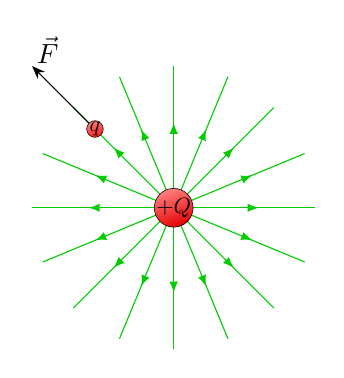
\begin{tikzpicture}
		\def\R{1.8}
		\def\NE{16}
		\def\NV{4}
		\contourlength{1.6pt}
		
		\foreach \i [evaluate={\angle=(\i-1)*360/\NE;}] in {1,...,\NE}{
			\draw[EFieldLineArrow={0.6}] (0,0) -- (\angle:\R);
		}
		\draw[charge+] (0,0) circle (7pt) node[black,scale=0.8] {$+Q$};
		%\draw[FFieldLineArrow={0.6}] (-1,1) -- (-2,2);
		\draw[-{Stealth[black]}] (-1,1) -- (-1.8,1.8) node at (-1.6, 2) {$\vec{F}$};
		\draw[charge_small] (-1,1) circle (3pt) node[black,scale=0.8] {$q$};
	\end{tikzpicture}
	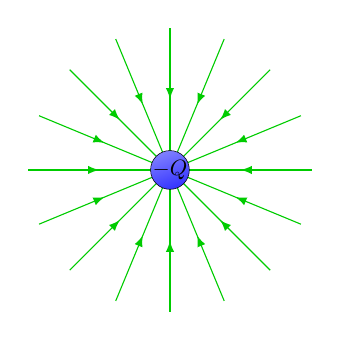
\begin{tikzpicture}
		\def\R{1.8}
		\def\NE{16}
		\def\NV{4}
		\contourlength{1.6pt}
		
		\foreach \i [evaluate={\angle=(\i-1)*360/\NE;}] in {1,...,\NE}{
			\draw[EFieldLineArrow={0.5}] (\angle:\R) -- (0:0);
		}
		\draw[charge-] (0,0) circle (7pt) node[black,scale=0.8] {$-Q$};
	\end{tikzpicture}
	\caption{Elektrisches Feld einer positiven-/ negativen Punktladung}
	\label{maxwell:section:E-Feld_punktladung}
\end{figure}

\subsubsection{Energiedichte im elektrischen Feld}
Das elektrische Feld beinhaltet eine Energie und somit auch eine Energiedichte.
Diese Energiedichte ist definiert als
\begin{equation}
w_e
=
\frac{1}{2} \epsilon \vec{E} ^2,
\label{maxwell:section:definiton_energiedichte_elektrischesFeld}
\end{equation}
wobei $\epsilon$ die Permittivität ist.
Die Permittivität
\[
\epsilon
=
\epsilon_r \epsilon_0
\]
ist das Produkt der relativen Permittivität $\epsilon_r$ und der Permittivität von Vakuum $\epsilon_0$.
Die relative Permittivität ist eine materialabhängige Grösse und hat in Vakuum den skalaren wert $1$.
Die Permittivität von Vakuum
\[
\epsilon_0
=
8.854 \cdot 10^{-12} F/m
\]
ist die elektrische Feldkonstante.


\subsection{Gausssches Gesetz quellenfrei
	\label{maxwell:section:elektrostatik_ohne_quelle}}
\rhead{Problemstellung}
Man stelle sich nun einen ladungsfreien, luftleeren, drei dimensionalen Raum $V\subset\mathbb{R}^3$
vor, indem ein elektrisches Potentialfeld $\phi(x,y,z)$ existiert.
Für diesen Raum möchten wir mittels der Varitaionsrechnung eine Gleichung entwickeln, die beschreibt, wie sich das Potentialfeld verhählt. 

\subsubsection{Ansatz}
Damit wir eine Gleichung erhalten, die das Verhalten des elektrischen Potentialfeldes beschreibt, muss ganz allgemein die Energie im System minimiert werden. 
In diesem Fall ist die Energie im System
\[
W_e
=
\iiint_V w_e\, dV.
\]
Dieses Integral gilt es zu minimieren, was die Grundlage für unser Variationsproblem darstellt.
Die in \eqref{maxwell:section:definiton_energiedichte_elektrischesFeld} definierte Energiedichte ist in Vakuum
% TODO: Bei definitionen erwähnen, dass ein vektor v^2 = v dot v ist!
\[
w_e\
=
\frac{1}{2}\epsilon_0\vec{E}(x,y,z)^2.
\]
Diese Gleichung können wir nun mittels definition \eqref{maxwell:section:definition_statisch_elektrischesFeld} mit dem elektrischen Potentialfeld ausdrücken.
somit ist
\begin{align}
\renewcommand{\arraystretch}{1.9}
w_e
&=
\frac{1}{2}\epsilon_0\left(-\nabla\phi(x,y,z)\right)^2
\\
w_e
&=
\frac{1}{2}\epsilon_0
\begin{pmatrix}
\displaystyle
-\phi_x\\
\displaystyle
-\phi_y\\
\displaystyle
-\phi_z
\end{pmatrix}
\cdot
\begin{pmatrix}
\displaystyle
-\phi_x\\
\displaystyle
-\phi_y\\
\displaystyle
-\phi_z
\end{pmatrix}
\\
w_e
&=
\frac{1}{2}\epsilon_0\left(\phi_x^2 + \phi_y^2 + \phi_z^2\right).
\label{maxwell:section:energiedichte}
\end{align}
Dies können wir in das zu minimerende Integral einsetzen und bekommen
%TODO: eventuell underbraces weg lassen.
\begin{equation}
	W_e
	=
	\iiint_V \underbrace{
		\frac{1}{2}\epsilon_0\left(\phi_x^2 + \phi_y^2 + \phi_z^2\right)}_{L(x,y,z,\phi,\phi_x,\phi_y,\phi_z)}\, dV.
	\label{maxwell:section:energieintegral_quellenfrei}
\end{equation}
Aus dieser Gleichung können wir entnehmen, dass unsere Lagrangefunktion
\begin{equation}
	L(x,y,z,\phi,\phi_x,\phi_y,\phi_z)
	=
	\frac{1}{2}\epsilon_0\left(\phi_x^2 + \phi_y^2 + \phi_z^2\right)
	\label{maxwell:section:lagrangefunktion_quellenfrei}
\end{equation}
ist.
Somit haben wir unsere Lagrangefunktion gefunden, die wir in einem nächsten Schritt in die Euler-Ostrogradski-Differentialgleichung einsetzen können.

\subsubsection{Einsetzen in die Euler-Ostrogradski-Differentialgleichung}
%TODO: label suchen von E-O-DGL von müller kapitel
Nun gilt es die in \eqref{maxwell:section:lagrangefunktion_quellenfrei} gefundene Gleichung in die E-O-DGL \ref{???} einzusetzen.
Nach Einsetzen wird die Differentialgleichung
\[
\frac{1}{2}\epsilon_0\left(\underbrace{\frac{\partial}{\partial\phi}\left(\phi_x^2 + \phi_y^2 + \phi_z^2\right)}_{=0} - \frac{\partial}{\partial x}\frac{\partial}{\partial \phi_x}\left(\phi_x^2 + \phi_y^2 + \phi_z^2\right) - 
\frac{\partial}{\partial y}\frac{\partial}{\partial \phi_y}\left(\phi_x^2 + \phi_y^2 + \phi_z^2\right) - 
\frac{\partial}{\partial z}\frac{\partial}{\partial \phi_z}\left(\phi_x^2 + \phi_y^2 + \phi_z^2\right)\right)
=
0.
\]
Man sieht, dass die partielle Ableitung nach $\phi$ verschwindet.
Nach den partiellen Ableitungen nach $\phi_x$, $\phi_y$ und $\phi_z$ wird die Differentialgleichung
\[
\frac{1}{2}\epsilon_0\left(-\frac{\partial}{\partial x}2\phi_x - \frac{\partial}{\partial y}2\phi_y - \frac{\partial}{\partial z}2\phi_z\right)
=
0.
\]
Wenn man nun noch die letzten partiellen Ableitungen macht, wird die Differentialgleichung
\begin{equation}
	- \underbrace{\epsilon_0}_{\not{=}0}\underbrace{\left(\frac{\partial^2\phi}{\partial x^2} + \frac{\partial^2\phi}{\partial y^2} + \frac{\partial^2\phi}{\partial z^2}\right)}_{=0}
	=
	0.
	\label{maxwell:section:laplace_gleichung_1}
\end{equation}
%definiton des laplace operators suchen
An dieser Gleichung sieht man, dass die Klammer mit den partiellen Ableitungen gleich null sein muss, da die Permittivität von Vakuum nicht null sein kann.
Zusätzlich wird nun ersichtlich, dass der Klammerterm nach definition \ref{???} mit dem Laplace-Operator angewendet auf das elektrische Potentialfeld $\phi$ ersetzt werden kann.
Somit wird unsere schluss Differentialgleichung
\begin{equation}
	\Delta\phi
	=
	0.
	\label{maxwell:section:laplace_gleichung_2}
\end{equation}
Durch Anwendng der Definiton des Laplace-Operator \ref{???} und der Definiton des elektrischen Feldes \eqref{maxwell:section:definition_statisch_elektrischesFeld} erhalten wird die Gleichung
\[
\nabla\cdot\underbrace{\nabla\phi}_{-\vec{E}}
=
0.
\]
Hiermit erhalten wir, dass
\begin{equation}
	\nabla\cdot\vec{E}
	=
	0
	\label{maxwell:section:e_feld_quellenfrei}
\end{equation}
% TODO:Bild referenz einfügen und Bild erstellen
sein muss. Diese Differentialgleichung besagt, dass das elektrische Feld quellenfrei ist.
Dies bedeutet, dass Felldlinien des elektrischen Feldes an keinem Ort im Raum enstehen oder enden können.
Dies ist sehr naheliegend, da ohne Ladungen im Raum das elektrische Feld quellenfrei sein muss.

%Darf auch weggelassen werden.
\subsubsection{Exkurs zur Laplace-Gleichung}
\label{maxwell:section:laplacegleichung_exkurs}
Ein Potentialfeld, das die Laplace-Gleichung
\[
-\Delta\varphi
=
0
\]
erfüllt, führt zu einem Gradientenfeld $\nabla\varphi$, das rotationsfrei und quellenfrei ist.
Diese Gleichung findet nicht nur Anwendungen in der Elektrostatik, sondern auch in stationärer Fluiddynamik und stationärer Wärmeleitung.







%
% einleitung.tex -- Beispiel-File für die Einleitung
%
% (c) 2020 Prof Dr Andreas Müller, Hochschule Rapperswil
%
% !TEX root = ../../buch.tex
% !TEX encoding = UTF-8
%
%erste Maxwell Gleichung mit Quelle
\subsection{Gausssches Gesetz
\label{maxwell:section:elektrostatik_mit_quelle}}
\rhead{Problemstellung}
Nun betrachten wir einen luftleeren, dreidimensionalen Raum $V\subset\mathbb{R}^3$, in dem ein elektrisches Potentialfeld $\phi(x,y,z)$ und eine Ladungsdichte $\varrho(x,y,z)$ existieren.
Auch für diesen Raum möchten wir mittels Variationsrechnung eine Gleichung finden, die das Verhalten des elektrischen Potentialfeldes beschreibt.

\subsubsection{Ansatz}
\rhead{Ansatz}
Es ist naheliegend, dass auch in diesem Szenario die Energie im System minimiert werden muss.
Wie auch in Gleichung \eqref{maxwell:section:energieintegral_quellenfrei} ist die Energie im elektrischen Feld
\[
W_e
=
\iiint_V \frac{1}{2}\,\varepsilon_0\,(\phi_x^2 + \phi_y^2 + \phi_z^2)\, dV.
\]
Jedoch ist dies nicht die einzige Komponente der gesamt Energie des Systems.
Laut \eqref{maxwell:section:definition_elektrischespotentialfeld} ist das elektrische Potential eine auf die Ladung normierte potentielle Energie.
Somit haben wir die fehlende Komponente gefunden.
Damit wir die durch die Ladung
\begin{equation}
q
=
\iiint_V \varrho(x,y,z)\, dV
\label{maxwell:ladung}
\end{equation}
verursachte potentielle Energie $W_q$ im System mit der Ladungsdichte $\varrho$ ausdrücken können, müssen wir untersuchen, was eine infinitesimale potentielle Energie verursacht.
Wenn wir diese infinitesimal kleine potentielle Energie
\(
dW_q
=
\phi\, dq
\)
unter die Lupe nehmen und für die infinitesimal kleine Ladung
\(
dq
=
\varrho\, dV
\)
einsetzen, erhalten wir
\(
dW_q
=
\phi\,\varrho\, dV.
\)
Jetzt müssen die infinitesimalen potentiellen Energien im Raum $V$ zusammengezählt werden und es resultiert
\begin{equation}
W_q
=
\iiint_V \varrho\,\phi\, dV.
\label{maxwell:section:potenzielle_energie_ladung}
\end{equation}
Mit der Gesamtenergie
\[
W_{tot}
=
W_e - W_q
=
\iiint_V \frac{1}{2}\,\varepsilon_0\left(\phi_x^2 + \phi_y^2 + \phi_z^2\right) - \phi\,\varrho\, dV
\]
des Systems haben wir unser zu minimierendes Integral gefunden.
Daraus können wir wieder die Lagrange-Funktion
\begin{equation}
L(x,y,z,\phi,\phi_x,\phi_y,\phi_z)
=
\frac{1}{2}\,\varepsilon_0\left(\phi_x^2 + \phi_y^2 + \phi_z^2\right) - \phi\,\varrho
\label{maxwell:section:lagrangefunktion_mit_quelle}
\end{equation}
% TODO: Müller fragen wegen kopplungsterme
ablesen.
Man bemerkt, dass die Lagrange-Funktion einen zusätzlichen additiven Term erhalten hat im Verlgeich zur Lagrange-Funktion \eqref{maxwell:section:lagrangefunktion_quellenfrei}.
Solche Terme nennt man Kopplungsterme.
Sie werden verwendet, um die Wechselwirkung zwischen Termen in der Lagrange-Funktion zu berücksichtigen.
Der Kopplungsterm in unserem Fall beschreibt die Wechselwirkung zwischen dem Feld und der Ladungsdichte.
Nun können wir diese Lagrangefunktion in die Euler-Ostrogradski-Differentialgleichung einsetzen, um zu untersuchen, wie sich das elektrische Potentialfeld verhält.

\subsubsection{Einsetzen in die Euler-Ostrogradski-Differentialgleichung}
Nun wollen wir die in \eqref{maxwell:section:lagrangefunktion_mit_quelle} gefundene Lagrangefunktion in die Euler-Ostrogradski-Differentialgleichung einsetzten.
Um die Rechnung übersichtlicher zu gestalten, machen wir uns die Linearität der Euler-Ostrogradski-Differentialgleichung
\begin{equation}
F\left\{W_{tot}\right\}
=
F\left\{W_e - W_q\right\}
=
F\left\{W_e\right\} + F\left\{-W_q\right\}
\label{maxwell:section:linearität_von_DGL}
\end{equation}
zu nutze.
Die Lösung von $F\left\{W_e\right\}$ haben wir in Gleichung \eqref{maxwell:section:laplace_gleichung_1} bereits gefunden.
Durch einsetzen von $-W_q$ in die Euler-Ostrogradski-Differentialgleichung erhalten wir
\[
\frac{\partial}{\partial\phi}\left(-\varrho\,\phi\right) - \underbrace{\frac{\partial}{\partial x}\frac{\partial}{\partial\phi_x}\left(\varrho\,\phi\right)}_{=0} - \underbrace{\frac{\partial}{\partial y}\frac{\partial}{\partial\phi_y}\left(\varrho\,\phi\right)}_{=0} - \underbrace{\frac{\partial}{\partial z}\frac{\partial}{\partial\phi_z}\left(\varrho\,\phi\right)}_{=0}
=
0.
\]
Da alle partiellen Ableitungen nach $\phi_x, \phi_y, \phi_z$ null ergeben, müssen wir nur noch die partielle Ableitung nach $\phi$ erledigen.
Somit ist
\(
-\varrho
=
0.
\)
Durch Addition unserer zwei Teillösungen erhalten wir die Gleichung
\begin{align*}
-\varepsilon_0\,\Delta\phi - \varrho
&=
0
\\
\Leftrightarrow \qquad \varepsilon_0\,\Delta\phi
&=
-\varrho.
\end{align*}
Schlussendlich erhalten wir
\begin{equation}
\Delta\phi
=
-\frac{\varrho}{\varepsilon_0}.
\label{maxwell:section:erste_maxwellgleichung_1}
\end{equation}
% TODO: definiton des laplace-operators suchen
Durch gleiches Vorgehen wie in Gleichung \eqref{maxwell:section:laplace_gleichung_3} erhalten wir
\[
\nabla\cdot\underbrace{\nabla\phi}_{\displaystyle-\vec{E}}
=
-\frac{\varrho}{\varepsilon_0}.
\]
Somit können wir erneut die Schlussdifferentialgleichung mit dem elektrischen Feld ausdrücken. Dadurch muss
\begin{equation}
\nabla\cdot\vec{E}
=
\frac{\varrho}{\varepsilon_0}
\label{maxwell:section:erste_maxwellgleichung_2}
\end{equation}
gelten.
Wir sehen, dass dies der ersten Maxwell-Gleichung in differentieller Schreibweise entspricht.

\subsubsection{Interpretation des Resultates}
Die erste Maxwell-Gleichung \eqref{maxwell:section:erste_maxwellgleichung_2} besagt, dass die Quelle des elektrischen Feldes eine Ladungsdichte $\varrho$ ist.
Dies bedeutet, dass elektrische Feldlinien auf Ladungen enden können.
In anderen Worten wird das elektrostatische Feld durch Ladungen erzeugt!
Da es sowohl positive wie auch negative Ladungen gibt, gilt dasselbe für die Ladungsdichten.
Wenn die Ladungsdichte positiv ist, sagt uns die erste Maxwell-Gleichung, dass das elektrische Feld eine Quelle besitzt.
Das heisst, salopp gesagt, die Feldvektoren zeigen weg von der Ladungsdichte.
Wenn die Ladungsdichte jedoch negativ ist, besitzt das elektrische Feld eine Senke.
Das heisst in diesem Fall, dass die Feldvektoren auf die Ladungsdichte zeigen. Dies ist in Abbildung \ref{maxwell:section:E-Feld_punktladung} veranschaulicht.

\subsubsection{Exkurs zur Poisson-Gleichung}
% Darf auch weggelassen werden.
Die Poisson-Gleichung
\[
\Delta\phi
=
f,
\]
wobei $\phi$ ein Potentialfeld und $f$ eine Quelle ist, findet in vielen Teilen der Physik ihre Anwendungen.
Die Quelle $f$ kann wie in Gleichung \eqref{maxwell:section:erste_maxwellgleichung_1} eine Funktion des Raumes und/oder eine Funkiton der Zeit sein.
Ein Potentialfeld, dass die Poisson-Gleichung erfüllt, führt zu einem Gradientenfeld $\nabla\varphi$, dass die Quelle $f$ besitzt und Rotationsfrei ist.
Die homogene Gleichung, also wo $f = 0$ ist, führt uns zur Laplace-Gleichung.








%
% magnetostatik.tex -- Herleitung Amperesches Gesetz über E-O-DGL
%
% (c) 2020 Prof Dr Andreas Müller, Hochschule Rapperswil
%
% !TEX root = ../../buch.tex
% !TEX encoding = UTF-8
%
\section{Magnetostatik\label{maxwell:magnetostatik}}
\rhead{Magnetostatik}



In der Magnetostatik betrachten wir stationäre magnetische Felder.
Die Ursache eines stationären magnetischen Feldes sind Permanentmagnete oder Gleichströme also bewegte Ladungen.
Wir setzen also neu
\[ 
\frac{\partial q}{\partial t}
=
I
=
\text{const}
\qquad
\forall
q,t
\]
voraus.
Zusätzlich konzentrieren wir uns in diesem Abschnitt ausschliesslich auf das magnetische Feld bzw. die magnetische Flussdichte, somit wird auch 
\[\phi(x,y,z) = 0 \qquad \forall x,y,z\] 
angenommen.

Fliesst ein konstanter Strom in einem Leiter, so erzeugt dieser ein Magnetfeld konzentrisch um den geraden Leiter, wie in Abbildung \ref{maxwell:flussdichte} abgebildet ist.
Aufgrund des nicht existieren magnetischer Monopole schliessen sich die Feldlinien des magnetischen Feldes vollständig, was bedeutet, dass das Feld keine Quellen aufweist und somit quellenfrei ist.

\begin{figure}
\centering
% WIRE B FIELD 3D
\begin{tikzpicture}[z={(0.8,0.28)},x={(0.58,-0.45)}]
	
	\def\L{6}
	\def\W{0.10}
	\def\R{0.9}
	\def\ang{-35}
	\def\scale{1.3}
	\def\NB{5}
	\coordinate (O) at (0,0,0);
	%\draw (0,0,0) -- (2,0,0);
	%\draw (0,0,0) -- (0,0,2);
	
	% Koordinatensystem
	\draw[->] (0,0,0) -- (3,0,0) node[anchor=north east]{$x$};
	\draw[->] (0,0,0) -- (0,3,0) node[anchor=north west]{$z$};
	\draw[->] (0,0,0) -- (0,0,4) node[anchor=south]{$y$};
	
	% B FIELD BACK
	\foreach \i [evaluate={\x=(\i-\NB/2-0.5)*\L/\NB;}] in {1,...,\NB}{
		%\draw[BField,-] (0,0,\x)++(\ang+1:\R) arc (\ang+1:\ang-181:\R);
		\draw[BFieldLine=1] (0,0,\x)++(\ang+1:\R) arc (\ang+1:\ang-181:\R) --++ (65:0.001*\R);
	}
	
	% WIRE
	\draw[metal] (0,0,-\L/2)++(120:\W/2) --++ (0,0,\L) arc (120:-60:\W/2) --++ (0,0,-\L) arc (-60:120:\W/2);
	\draw[metal] (0,0,-\L/2) circle (\W/2);
	\draw[current] (0.12*\R,-0.12*\R,0.4*\L) --++ (0,0,0.2*\L) node[below=2,right] {$I$};
	
	% B FIELD FRONT
	\foreach \i [evaluate={\x=(\i-\NB/2-0.5)*\L/\NB;}] in {1,...,\NB}{
		%\draw[BFieldLine=1] (0,0,\x)++(\ang+180:\R) arc (\ang+180:\ang:\R) --++ (-116:0.001*\R);
		\draw[BField,-] (0,0,\x)++(\ang+180:\R) arc (\ang+180:\ang:\R);
	}
	\node[Bcol] at (-0.9*\R,0.9*\R,-0.25*\L) {$\vec{B}$}; %++(140:1.3*\R)
	
\end{tikzpicture}
	\caption{Magnetische Flussdichte um einen geraden Leiter}
	\label{maxwell:flussdichte}
\end{figure}




\subsubsection{Magnetisches Vektorpotential}

Das magnetische Vektorpotential ist ein Vektorfeld, mit welchem die magnetische Flussdichte als 
\begin{equation}
	\nabla \times \vec{A}
	=
	\vec{B}
	\label{maxwell:definitionVektorpot}
\end{equation}
beschreiben werden kann, wobei wir für später dieses bereits konkret ausrechnen wollen 
\begin{equation}
	\renewcommand{\arraystretch}{1.9}
	\begin{pmatrix}
		\displaystyle
		\frac{\partial}{\partial x} \\
		\displaystyle
		\frac{\partial}{\partial y} \\
		\displaystyle
		\frac{\partial}{\partial z}
	\end{pmatrix}
	\times
	\begin{pmatrix}
		\displaystyle
		A_1 \\
		A_2 \\
		A_3 \\
	\end{pmatrix}
	=
	\begin{pmatrix}
		\displaystyle
		\frac{\partial A_3}{\partial y} -\frac{\partial A_2}{\partial z}\\
		\displaystyle
		\frac{\partial A_1}{\partial z} -\frac{\partial A_3}{\partial x}\\
		\displaystyle
		\frac{\partial A_2}{\partial x} -\frac{\partial A_1}{\partial y}
	\end{pmatrix}.
\end{equation}

Mit dem Vektorpotential können ähnlich wie beim elektrischen Potential, energetische Zustände beschrieben werden. Die Wirkgrösse hier ist allerdings eine bewegte Ladung also eine Ladung $q$, welche eine Geschwindigkeit $\vec{v}$ hat. So kann das magnetische Potential dieser Grösse an einem Punkt berechnet werden. Zusätzlich ergibt sich über das Vektorpotential so auch die potentielle Energie dieser Wirkgrösse, auf welche weiter unten noch spezifischer eingegangen wird.


\subsection{Ampère'sches Gesetz}

Wiederum betrachten wir unter den oben vorausgesetzten Bedingungen einen luftleeren, dreidimensionalen Raum $V \subset \mathbb{R}^3$ in welchem das Vektorfeld des magnetischen Vektorpotentials $\vec{A}(x,y,z)$ und eine Stromdichte $\vec{j}(x,y,z)$ existieren. Erneut versuchen wir eine Gleichung zu finden, welche das Wesen des Vektorpotential und somit nach \ref{maxwell:definitionVektorpot} die magnetische Flussdichte bzw. das magnetische Feld beschreibt. 

\subsubsection{Ansatz}

Wieder soll die Energie des gesamten Systems minimiert werden. 
Die Energiedichte des magnetischen Feldes mit \ref{maxwell:definitionVektorpot} eingesetzt ist
\[ w_m 
= 
\frac{1}{2\mu_0}\vec{B}(x,y,z)^2
=
\frac{1}{2\mu_0}\left(\nabla\times\vec{A}(x,y,z)\right)^2. \]
Somit berechnet sich die gesamt Energie jenes zu 
\begin{equation}
	W_m = \iiint_V w_m\, dV.
\end{equation}
Wie bereits erwähnt, ergibt sich durch eine bewegte Ladung $q$ mit einer Geschwindigkeit $\vec{v}$ eine weitere potentielle Energie im System, welche sich als 
\[ 
W_{p}
= 
\vec{A}
\cdot
q\vec{v}
 \]
berechnen lässt.
Mithilfe von $\vec{j} = \rho\vec{v}$ und \ref{maxwell:ladung} kann diese potentielle Energie zu 
\begin{equation}
	W_p
	= 
	\iiint_V \vec{A}(x,y,z)\cdot\vec{j}(x,y,z)\,dV
\end{equation}
umgeformt werden.
Die beiden Komponenten welche einen Beitrag zur gesamt Energie beitragen können so als 
\begin{align*}
W_{tot} 
&=
W_m - W_p
=
\iiint_V \vec{A}\cdot\vec{j}
- \frac{1}{2\mu_0}\left(\nabla\times\vec{A}\right)\cdot\left(\nabla\times\vec{A}\right)\, dV \\
&=
\iiint_V \left( A_1j_1 + A_2j_2 + A_3j_3\right) - 
 \frac{1}{2\mu_0}\left( 
 	\left( \frac{\partial A_3}{\partial y} -\frac{\partial A_2}{\partial z}\right)^2 
 + \left( \frac{\partial A_1}{\partial z} -\frac{\partial A_3}{\partial x}\right)^2
 + \left(\frac{\partial A_2}{\partial x} -\frac{\partial A_1}{\partial y} \right)^2   
 \right) \,dV
\end{align*}
zusammengefasst werden. 

In dieser Gleichung wird sofort das zu minimierende Integral ersichtlich und die Lagrange Funktion kann als 

	%\begin{align}
	%\label{maxwell:magnetostatikLagrange}
	%L\left(x,y,z, \vec{A}, \vec{A}_x. \vec{A}_y, \vec{A}_z\right)
	%=&\left( A_1j_1 + A_2j_2 + A_3j_3\right) \\ \nonumber
	% &- \frac{1}{2\mu_0}\left( 
	%\left( \frac{\partial A_3}{\partial y} -\frac{\partial A_2}{\partial %z}\right)^2 
	%+ \left( \frac{\partial A_1}{\partial z} -\frac{\partial A_3}{\partial x}\right)^2
	%+ \left(\frac{\partial A_2}{\partial x} -\frac{\partial A_1}{\partial y} \right)^2   
	%\right)	
	%\end{align}
	
	\begin{align}
	\label{maxwell:magnetostatikLagrange}
	L\left(x,y,z, \vec{A}, \vec{A}_x. \vec{A}_y, \vec{A}_z\right)
	=&\left( A_1j_1 + A_2j_2 + A_3j_3\right) \\ \nonumber
	 &- \frac{1}{2\mu_0}\left( 
	\left( A_{3y} - A_{2z}\right)^2 
	+ \left(A_{1z} -A_{3x}\right)^2
	+ \left(A_{2x} -A_{1y}\right)^2   
	\right)
	\end{align}
definiert werden. 
Hierbei wollen wir darauf hinweisen, dass die Lagrange Funktion in diesem Fall von einem Vektor abhängig ist. 
Das bedeutet, dass jede Komponente des Vektorpotentials einzeln variiert werden kann, was später die Ursache für mehrere Ausführungen der E-O-DGL sein wird.

Erneut stellen wir auch fest, dass ein additiver Term dazugekommen ist, wie weiter oben beschrieben handelt es sich auch hier um einem Koppelungsterm, welcher hier jedoch die Wechselwirkung zwischen dem Feld und der Wirkgrösse also der Stromdichte $\vec{j}$ beschreibt.

\subsubsection{Einsetzen in die Euler-Ostrogradski-Differentialgleichung}

Da jede Komponente des magnetischen Vektorpotentials für sich variiert werden kann, resultieren demnach drei E-O-DGL der Form
\[ 
\frac{\partial L}{\partial A_i} 
- \frac{\partial}{\partial x}\frac{\partial L}{\partial A_{ix}}
- \frac{\partial}{\partial y}\frac{\partial L}{\partial A_{iy}}
- \frac{\partial}{\partial z}\frac{\partial L}{\partial A_{iz}}
= 0 \qquad \text{für } i=1,2,3
 \]
{\larger\textcircled{\smaller[2]1}} $i = 1$
\begin{subequations}
\begin{gather}
	0
	=
	j_1 - \underbrace{\frac{\partial}{\partial x}\frac{\partial L}{\partial A_{1x}}}_{=0}
	 - \left( \frac{1}{2\mu_0}(-1)\,2 \frac{\partial}{\partial y}(A_{2x}-A_{1y})\right) 
	 - \left( \frac{1}{2\mu_0}\,2\frac{\partial}{\partial z}(A_{1z}-A_{3x})\right)
	 \\
	 0
	 =
	 j_1 - \frac{1}{\mu_0}\left( \frac{\partial}{\partial y}(A_{2x}-A_{1y})
	 - \frac{\partial}{\partial z}(A_{1z}-A_{3x})
	 \right)  
	 \\	 
	 \mu_0j_1
	 =
	 \frac{\partial}{\partial y}(A_{2x}-A_{1y})
	 - \frac{\partial}{\partial z}(A_{1z}-A_{3x})	 	 	 
\end{gather}
\end{subequations}


%%
% einleitung.tex -- Beispiel-File für die Einleitung
%
% (c) 2020 Prof Dr Andreas Müller, Hochschule Rapperswil
%
% !TEX root = ../../buch.tex
% !TEX encoding = UTF-8
%
\section{Einleitung\label{circuit:section:teil0}}
\rhead{Einleitung}
Das folgende kapitel beschäftig sich mit der Frage wie man elektronische DC Schaltungen ohne die zuhilfenahme von Kirchhoff's gesetzen lösen kannm mit hilfe von Variationsrechnungen.  \cite{circuit:bibtex}.





%%
% teil1.tex -- Beispiel-File für das Paper
%
% (c) 2020 Prof Dr Andreas Müller, Hochschule Rapperswil
%
% !TEX root = ../../buch.tex
% !TEX encoding = UTF-8
%
\section{Kirchhoffs Gesetz
\label{circuit:section:teil1}}
\rhead{Problemstellung}
Bevor wir die Laplace-Gleichung mithilfe der Lagrange-Funktion herleiten, versuchen wir das auf konventionelle Weise, indem wir  das kirchhoffsche Gesetz benutzen. 
Dafür brauchen wir aber zuerst noch ein paar Erkenntnisse, die hier aufgezeigt werden. Die Stromdichte $\vec{J}$ wird durch
\begin{equation}
	\vec{J}=\frac{\vec{I}}{A}
	\label{circuit:current_density_3}
\end{equation}
definiert. Diese Gleichung besagt, dass die Stromdichte das Verhältnis des Stroms $\vec{I}$ zur Flächen $A$ ist. 
Das kirchhoffsche Stromgesetz postuliert nun, dass die Summe der in einen Knoten einfliessenden Ströme gleich der Summe der aus diesem Knoten ausfliessenden Ströme in einer Schaltung ist. Dies impliziert, dass es in einem Gleichstromkreis im stationären Zustand keine Ladungsakkumulation an irgendeinem Punkt geben kann. Wir betrachten nun einen dreidimensionalen Schaltkreis, in dem die Leitfähigkeit $\sigma$ im gesamten Bereich von Interesse konstant ist. Die Verallgemeinerung des kirchhoffschen Stromgesetzes im dreidimensionalen Fall besagt, dass die Divergenz der Stromdichte $\vec{J}$ gleich Null ist, es kann kein Strom aus dem Nichts erzeugt werden. Daher gilt 
%\eqref{circuit:current_density_1}.
\begin{equation}
	\nabla \cdot  \vec{J}=0.
	\label{circuit:current_density_1}
\end{equation}

Zudem lässt sich der Zusammenhang zwischen dem elektrischen Feld $\vec{E}$ an einem gegebenen Punkt im Raum als negativer Gradient 
\begin{equation}
	\vec{E}=-\nabla \phi
	\label{circuit:current_density_4}
\end{equation}
der Potentialfunktion $\phi$ ausdrücken.

Wenn das elektrische Feld durch $\vec{E}$ repräsentiert wird und wir ein ohmsches Material vorliegen haben, kann die Stromdichte auch als Produkt  
\begin{equation}
\vec{J}=\sigma \vec{E}
\label{circuit:current_density_2}
\end{equation}
beschrieben werden.
Mit dem elektrischen Feld als Gradient von $\phi$ erhalten wir aus der Quellenfreiheit des Stromes \eqref{circuit:current_density_1} und dem ohmschen Gesetz \eqref{circuit:current_density_2} die Differentialgleichung 
\begin{equation}
	\nabla \cdot (\sigma \nabla \phi)=0
	\label{circuit:current_density_5}
\end{equation}
für das Potential $\phi$. Dies kann auch als
\begin{equation}
\nabla^2 \phi=0
\label{circuit:current_density_6}
\end{equation}
geschrieben werden, solange $\sigma$ konstant ist.

\section{Variationsprinzip} 
In diesem Abschnitt wird das Ziel verfolgt, die Gleichung \eqref{circuit:current_density_6} mithilfe eines Variationsprinzips herzuleiten und seine Bedeutung aufzuzeigen. Zunächst werden jedoch die Grundlagen anhand eines einfachen Beispiels wiederholt.
\begin{figure}
	\centering
	\begin{circuitikz}
		\draw (0,3) to[V, v=$U_0$, i=$I_0$] (0,0);
		\draw (0,3) to[short,-*] (3,3)
		to[R, l=$R_1$, i=$I_1$] (3,0) -- (0,0);
		\draw (3,3) -- (6,3)
		to[R, l=$R_2$, i=$I_2$] (6,0) to[short,-*] (3,0);
	\end{circuitikz}
	\caption{Parallelschaltung von $R_1= \SI{2}{\kilo\ohm}$ und $R_2= \SI{1}{\kilo\ohm}$}
	\label{fig:circuit_stromzweig}
\end{figure}

\subsection{Berechnung der Stromverteilung mit klassischen Mitteln} 
Die klassische Methode zur Berechnung der Stromverteilung in einer Parallelschaltung von Widerständen basiert auf dem Ohmschen Gesetz und den Kirchhoffschen Regeln. Das Ohmsche Gesetz lautet:

\begin{equation}
	U=R \cdot I
	\label{circuit:ohmic_law}
\end{equation}

Die Kirchhoffschen Regeln besagen, dass in einem Knotenpunkt eines elektrischen Netzwerkes die Summe der zufliessenden Ströme gleich der Summe der abfliessenden Ströme ist und dass alle Teilspannungen eines Umlaufs bzw. einer Masche in einem elektrischen Netzwerk sich zu null addieren \cite{dewiki:244855415}. Mit diesen Regeln kann man direkt die Ströme in Abbildung \ref{fig:circuit_stromzweig} berechnen und erhält:

\begin{equation}
	I_1 = \frac{I_0 \cdot R_2}{R_1 + R_2} = \frac{\SI{1}{\ampere} \cdot \SI{1}{\kilo\ohm}}{\SI{2}{\kilo\ohm}+ \SI{1}{\kilo\ohm}}=\SI{0.333}{\ampere}
	\label{circuit:current_circuit_power_example3}
\end{equation}

\begin{equation}
	I_2 = I_0-I_1=\SI{1}{\ampere}-\SI{0.333}{\ampere}=\SI{0.667}{\ampere}
	\label{circuit:current_circuit_power4}
\end{equation}
unter der Bedingung das $I_0=\SI{1}{\ampere}$.

Diese Berechnung scheint auf den ersten Blick einfach zu sein, doch es gibt auch eine alternative Methode, das Minimalprinzip, das zum gleichen Ergebnis führt.

\subsection{Das Minimalprinzip als Alternative} 
Das Minimalprinzip bietet eine alternative Methode zur Berechnung der Stromverteilung. Es besagt, dass ein physikalisches System so arbeitet, dass eine bestimmte Größe minimiert wird. In unserem Fall ist diese Größe die Leistung der Schaltung, die durch die Formel
\begin{equation}
	P(I_1)=  I_1^2 \cdot R_1+  (I_0-I_1)^2 \cdot R_2
	\label{circuit:current_circuit_power}
\end{equation}
ausgedrückt wird. Um das Minimum zu finden, leiten wir die Leistung nach $I_1$ ab und setzen die Ableitung gleich Null. Dies führt zu:
\begin{equation}
	\frac{dP}{dI_1} = 2\cdot I_1\cdot R_1 - 2\cdot (I_0 - I_1) \cdot R_2.
	\label{circuit:current_circuit_power1}
\end{equation}
Die zweite Ableitung 
\begin{equation}
	\frac{d^2P}{dI_1^2} = 2\cdot R_1 + 2\cdot R_2
	\label{circuit:current_circuit_power2}
\end{equation}
zeigt eindeutig, dass es sich um ein Minimum handelt, da $R_1$ und $R_2$ positiv sind und daher die zweite Ableitung positiv ist. Wenn wir nun die erste Ableitung \eqref{circuit:current_circuit_power1} gleich Null setzen und auf $I_1$ auflösen bekommen wir
\begin{equation}
	I_1 = \frac{I_0 \cdot R_2}{R_1 + R_2} = \frac{\SI{1}{\ampere} \cdot \SI{1}{\kilo\ohm}}{\SI{2}{\kilo\ohm}+ \SI{1}{\kilo\ohm}}=\SI{0.333}{\ampere}
	\label{circuit:current_circuit_power_a}
\end{equation}
und analog dazu
\begin{equation}
	I_2 = I_0-I_1=\SI{1}{\ampere}-\SI{0.333}{\ampere}=\SI{0.667}{\ampere},
	\label{circuit:current_circuit_power_b}
\end{equation}
wie auch schon in in Gleichung \eqref{circuit:current_circuit_power_example3} und Gelichung \eqref{circuit:current_circuit_power4}.

Dies demonstriert erfolgreich, dass die Verteilung des Stroms in der Schaltung direkt mit der Minimierung der gesamten Leistung korrespondiert. Dies kann auch grafisch wie in Abbildung \ref{fig:circuit_power} dargestellt werden.

\begin{figure}
	\centering
	\includegraphics[width=0.7\textwidth]{papers/circuit/two_parrallel_resistors.png}
	\caption{Leistung ($z$-Achse) von zwei parallel geschalteten Widerständen 1 Kilo Ohm ($x$-Achse) und 2 Kilo Ohm ($y$-Achse), in grau dargestellt die Schnittfläche des Stromes von einem Ampere.}
	\label{fig:circuit_power}
\end{figure}

\subsection{Verallgemeinerung auf den stetigen Fall}
Die obige Analyse kann auf den stetigen Fall verallgemeinert werden, indem die Leistung $P$ in einem von einer Oberfläche $S$ umgebenen Volumen $V$ durch 
\begin{equation}
	P=\int_V \sigma(\nabla \phi)^2 d V
	\label{circuit:current_density_7}
\end{equation}
ausdrücken. Wenn wir nun die Euler-Ostrogradski-Differentialgleichung für \eqref{circuit:current_density_7} bestimmen und lösen, gibt uns dies anschliessend die Lösung für die minimale Leistung in einem zweidimensionalen oder dreidimensionalen Raum. D. h. um das Minimum zu finden muss das Integral von \eqref{circuit:current_density_7} minimiert werden. Auf den ersten Blick mag \eqref{circuit:current_density_7} nicht sehr intuitiv erscheinen. Daher könnten wir die Gleichung auch anders formulieren, wie in 
\begin{equation}
	P=\frac{U^2}{R}
	\label{circuit:current_density_8}
\end{equation}
gezeigt, wobei $U^2=\left( \nabla \phi \right)^2$ und $R=\frac{1}{\sigma}$.





%
%
%
%Analog zu dem oben aufgeführten Beispiel können wir die Leistung $P$ in einem von einer Oberfläche $S$ umgebenen Volumen $V$ durch 
%\begin{equation}
%	P=\int_V \sigma(\nabla \phi)^2 d V
%	\label{circuit:current_density_7}
%\end{equation}
%ausdrücken. Wenn wir nun die Euler-Ostrogradski-Differentialgleichung für \eqref{circuit:current_density_7} bestimmen und lösen gibt uns dies anschliessend die Lösung für die minimale Leistung in einem zweidimensionalen oder dreidimensionalen Raum. D.h. um das Minimum zu finden muss das Integral von \eqref{circuit:current_density_7} minimiert werden. Auf den ersten Blick mag \eqref{circuit:current_density_7} nicht sehr intuitiv erscheinen. Daher könnten wir die Gleichung auch anders formulieren, wie in 
%\begin{equation}
%	P=\frac{U^2}{R}
%	\label{circuit:current_density_8}
%\end{equation}
%gezeigt, wobei $U^2=\left( \nabla \phi \right)^2$ und $R=\frac{1}{\sigma}$.


\section{Herleitung der Laplace-Gleichung}
In diesem Kapitel leiten wir die Laplace-Gleichung her. Die Herleitung basiert auf der Euler-Ostrogradski-Differentialgleichung, die in Gleichung \eqref{buch:felder:ostrogradski:eqn:euler-ostrogradski} dargestellt ist.

Wir beginnen mit Gleichung \eqref{circuit:current_density_7} und wenden darauf die genannte Differentialgleichung an:
\begin{enumerate}
	\item Schritt: Lagrange-Funktion des Problems ohne $\sigma$ (da wir das Minimum suchen und $\sigma$ eine Konstante ist hat $\sigma$ keinen Einfluss auf die Lösung und kann daher weggelassen werden)
	\begin{equation}
		L(U, U_x)= U_x^2 = (U_{x_1}^2+U_{x_2}^2).
	\end{equation}
	\item Schritt: partielle Ableitungen
	\begin{equation}
		\begin{aligned}
			\frac{\partial L}{\partial U}&=0\\
			\frac{\partial L}{\partial U_{x_1}}&=2U_{x_1}\\
			\frac{\partial L}{\partial U_{x_2}}&=2U_{x_2}.\\
		\end{aligned}
	\end{equation}
	\item Schritt: Ableiten nach $x_1$ und $x_2$
	\begin{equation}
		\begin{aligned}
			\frac{\partial}{\partial x_1}\frac{\partial L}{\partial U_{x_1}}(x,\phi,\nabla \phi)=2\frac{\partial \phi}{\partial {x_1}}\cdot \frac{\partial}{\partial x_1},\\
			\frac{\partial}{\partial x_2}\frac{\partial L}{\partial U_{x_2}}(x,\phi,\nabla \phi)=2\frac{\partial \phi}{\partial {x_2}} \cdot \frac{\partial}{\partial x_1}.\\
		\end{aligned}
	\end{equation}
	\item Schritt: Euler-Ostrogradski Differentialgleichung
	\begin{equation}
		0=-\frac{\partial}{\partial x_1}\cdot 2\frac{\partial \phi}{\partial {x_1}}-\frac{\partial}{\partial x_2}\cdot 2\frac{\partial \phi}{\partial {x_2}}=-2\Delta\phi.
	\end{equation}
\end{enumerate}

Das Ergebnis der Anwendung der Theorie der Euler-Ostrogradski-Differentialgleichung ist:
	\begin{equation}
	\sigma \cdot 2\Delta\phi=0.
	\end{equation}
Wir können nun noch durch $2\sigma$ teilen und erhalten die Laplace-Gleichung aus \eqref{circuit:current_density_6}. Somit wurde gezeigt, dass die Laplace-Gleichung sowohl durch das Variationsprinzip als auch durch die Kirchhoffschen Regeln gefunden werden kann.



\section{Praktische Anwendungen}
In diesem Abschnitt werden wir die numerische Lösung der elliptischen partiellen Differentialgleichung \eqref{circuit:current_density_6} untersuchen und ihre Bedeutung erläutern.

\subsection{Diskretisierung der Ableitungen} Die Gleichung \eqref{circuit:current_density_6} kann durch eine Differenz zweiter Ordnung diskretisiert werden, wie in Gleichung \eqref{circuit:second-order-central} dargestellt:

\begin{equation}
	f^{\prime \prime}(x) \approx \frac{\delta_h^2[f](x)}{h^2}=\frac{\frac{f(x+h)-f(x)}{h}-\frac{f(x)-f(x-h)}{h}}{h}=\frac{f(x+h)-2 f(x)+f(x-h)}{h^2}.
	\label{circuit:second-order-central}
\end{equation}
\cite{enwiki:1220817436}

\subsection{Diskretisierung in zwei Dimensionen} Um diese Diskretisierung auf unseren zweidimensionalen Fall anzuwenden, führen wir ein Gitter ein, dessen Punkte durch die Koordinaten $(x_i, y_j)$ repräsentiert werden. Die Differenzen zwischen den Gitterpunkten in x- und y-Richtung werden durch $\Delta x$ und $\Delta y$ dargestellt. Dies führt zu folgender diskretisierter Gleichung:
\begin{equation}
	\frac{\phi(x_{i+1}, y_j) - 2\phi(x_i, y_j) + \phi(x_{i-1}, y_j)}{(\Delta x)^2} + \frac{\phi(x_i, y_{j+1}) - 2\phi(x_i, y_j) + \phi(x_i, y_{j-1})}{(\Delta y)^2} = 0.
	\label{circuit:discret_equation}
\end{equation}

\subsection{Auflösen nach $\phi(x_i, y_j)$} 
Wir können nun nach $\phi(x_i, y_j)$ auflösen und erhalten:
\begin{equation}
	\phi(x_i, y_j) = \frac{1}{4}(\phi(x_{i+1}, y_{j}) + \phi(x_{i-1}, y_{j}) + \phi(x_{i}, y_{j+1}) + \phi(x_{i}, y_{j-1})).
	\label{circuit:discret_equation2}
\end{equation}
Diese Gleichung ermöglicht es uns, das Potential an jedem Gitterpunkt zu berechnen, indem wir die Potentiale der umliegenden Punkte verwenden. Die Form von \eqref{circuit:discret_equation2} ist eine andere Darstellung von \eqref{circuit:discret_equation} für die numerische Implementierung.

\subsection{Numerisches Beispiel} 
\subsubsection{Quadratisches Kontakt}
Betrachten wir als Beispiel eine leitende Platte mit einer Leitfähigkeit von \SI{0.001}{\siemens\per\meter} und einer Größe von einem Quadratmeter. Ein spezifischer Bereich der Platte, Quadrat definiert durch $0.5 < x < 0.7$ und $0.5 < y < 0.7$, wird mit einem Potential von einem Volt belegt, während der Rand der Platte ein Potential von 0 Volt aufweist.

\begin{figure}
	\centering
	\includegraphics[width=0.99\textwidth]{papers/circuit/potential_distribution.png}
	\caption{Potential-Verteilung auf rechteckiger Platte mit rechteckigem Potential im oberen rechten Bereich und 0 Potential am Rand der Platte \cite{github:AndreasFMueller}}
	\label{fig:potential_distribution}
\end{figure}
Unter Verwendung von Gleichung \eqref{circuit:discret_equation2} zur Berechnung des Potentials und den gegebenen Randbedingungen erhalten wir die in Abbildung \ref{fig:potential_distribution} dargestellte Potentialverteilung. Dies ermöglicht uns, das gesamte Potential auf der Platte zu bestimmen.

Sobald das Potential bekannt ist, können wir mithilfe des Gradienten und Gleichung \eqref{circuit:current_density_7} die Leistungsdichte an jedem einzelnen Punkt berechnen. Dies führt zu den in Abbildung \ref{fig:power_2d} und \ref{fig:power_3d_rectangle} dargestellten Leistungsdichteverteilung.
\begin{figure}[h]
	\centering
	\includegraphics[width=0.99\textwidth]{papers/circuit/power_distribution.png}
	\caption{Leistungsdichte auf rechteckiger Platte mit rechteckigem Potential im oberen rechten Bereich und 0 Potential am Rand der Platte. (Code für die Generierung des Plots kann in \cite{github:AndreasFMueller} gefunden werden.)}
	\label{fig:power_2d}
\end{figure}
\begin{figure}[h]
	\centering
	\includegraphics[width=0.99\textwidth]{papers/circuit/power_distribution_circle.png}
	\caption{Leistungsdichte auf rechteckiger Platte mit kreisförmigen Potential im oberen rechten Bereich und 0 Potential am Rand der Platte. (Code für die Generierung des Plots kann in \cite{github:AndreasFMueller} gefunden werden.)}
	\label{fig:power_2d_circle}
\end{figure}
\begin{figure}[h]
	\centering
	\includegraphics[width=0.99\textwidth]{papers/circuit/3d.png}
	\caption{Leistungsdichte 3d auf rechteckiger Platte mit rechteckigem Potential und 0 Potential am Rand der Platte. (Code für die Generierung des Plots kann in \cite{github:AndreasFMueller} gefunden werden.)}
	\label{fig:power_3d_rectangle}
\end{figure}
\begin{figure}[h]
	\centering
	\includegraphics[width=0.99\textwidth]{papers/circuit/3d_circle.png}
	\caption{Leistungsdichte 3d auf rechteckiger Platte mit kreisförmigen Potential und 0 Potential am Rand der Platte. (Code für die Generierung des Plots kann in \cite{github:AndreasFMueller} gefunden werden.)}
	\label{fig:power_3d_circle}
\end{figure}
Abbildung \ref{fig:power_3d_rectangle} zeigt deutlich, dass die Leistungsdichte in den Ecken des zuvor definierten quadratischen Potentials am höchsten ist. Dies ist unter anderem ein Grund, warum auf Leiterplatten normalerweise keine 90°-Winkel für Leiterbahnen gezeichnet werden, sondern meistens 45°-Winkel verwendet werden, um die Leistungsdichte bzw. Stromdichte in den Ecken zu minimieren.

\subsubsection{Kreisförmiges Kontakt} Wenn wir anstelle eines rechteckigen Potentials ein kreisförmiges Potential verwenden, ist die Leistungsdichte deutlich geringer, wie in Abbildung \ref{fig:power_3d_circle} und Abbildung \ref{fig:power_2d_circle} dargestellt. Daher ist es vorteilhaft, abgerundete Ecken zu verwenden, wenn man die Leistungsdichte auf einer Leiterbahn minimieren möchte.

Diese Beispiele illustrieren die praktische Anwendung des Variationsprinzips und der numerischen Lösung von partiellen Differentialgleichungen in der Elektrotechnik. Sie zeigen, wie die Form von Leiterbahnen auf einer Leiterplatte optimiert werden können, um die Leistungsdichte zu minimieren und die Effizienz zu maximieren.
%%
% teil2.tex -- Beispiel-File für teil2 
%
% (c) 2020 Prof Dr Andreas Müller, Hochschule Rapperswil
%
% !TEX root = ../../buch.tex
% !TEX encoding = UTF-8
%
\section{Herleitung der Balkengleichung
	\label{balken:section:teil2}}
\subsection{Variationsprinzip}
Die Variationsrechnung ist ein Teilgebiet der Analysis, das sich mit kleinen Änderungen in Funktionen und Funktionalen beschäftigt, um Minima und Maxima von Funktionen zu ermitteln. Dabei handelt es sich um mathematische Ausdrücke, die Integrale über eine unbekannte Funktion und ihre Ableitung darstellen können. Ziel ist es, ein Maximum, ein Minimum oder einen Sattelpunkt ausfindig zu machen.

In der Mechanik kommen Variationsrechnungen oft zum Einsatz, da sie die Grundlage aller physikalischen Extremalrechnungen bilden. \ref{balken:Variationsrechnung}

\subsection{Minimalprinzip}
Das Minimalprinzip ist ein Konzept, das besagt, dass ein physikalisches System einen Zustand annimmt, der mit dem geringsten Energieaufwand erreicht wird. In der Physik wird das Minimalprinzip oft formuliert, indem eine minimale Wirkung oder Energie angestrebt wird.

Ein Beispiel hierfür ist eine Feder, die an einem Ende an einer Wand befestigt ist und an ihrem anderen Ende eine Masse trägt. Zieht man die Masse nach unten und lässt sie los, nimmt sie eine Position ein, bei der die potenzielle Energie minimal ist.

Das Minimalprinzip in Bezug auf die Balkengleichung ist ein grundlegendes Konzept der Mechanik, auch bekannt als das Prinzip von Hamilton. Es besagt, dass ein System den Gleichgewichtszustand annimmt, bei dem die potenzielle Energie minimal ist. Für einen Balken tritt dieser Zustand ein, wenn alle äusseren Kräfte, Momente, inneren Beanspruchungen sowie Verformungen des Balkens im Gleichgewicht stehen. Die Anwendung dieses Minimalprinzips führt zur Balkengleichung, die die Gleichgewichtsbedingungen des Balkens beschreibt. 

\subsection{Herleitung der Balkengleichung aus dem Variationsprinzip}
Die Verformungen des Balkens aufgrund der auftretenden Biegespannungen $σ_x$ werden durch
\begin{equation}
	\sigma_x = \frac{E}{p} z
\end{equation}
und
\begin{equation}
	\sigma_x = \frac{M_y}{I_y} z
\end{equation}
beschrieben. Setzt man diese beiden Gleichungen gleich, erhält man
\begin{equation}
	\frac{E}{p} z = \frac{M_y}{I_y} z
\end{equation}
und kürzt anschliessend $z$ heraus, so bekommt man
\begin{equation}
	\frac{E}{p} = \frac{M_y}{I_y}
\end{equation}
Dividiert man diese Gleichung durch $E$, um $p$ zu isolieren, erhält man die Formel für den Krümmungsradius
\begin{equation}
	\frac{1}{p} = \frac{M_y}{E I_y} = \kappa
\end{equation}

Bei Biegungen, die aufgrund von Querkräften auftreten, ist das Moment veränderlich und hängt von der Position $x$ ab. Dies führt dazu, dass die Krümmung des Balkens bzw. der Biegelinie von der Position $x$ abhängt. Um die Krümmung zu bestimmen, benötigt man den kürzesten Weg zwischen beiden Auflagern des Balkens.
\begin{figure}[h]
	\centering
	\includegraphics[width=0.8\textwidth]{papers/balken/images/teil2/BiegungBalke2.jpg}
	\caption{Darstellung der Biegelinie $y(x)$ mit dem Balken (rot gekennzeichnet) und dessen Auflagern.}
	\label{fig:Darstellung_der_Biegelinie}
\end{figure}

Zuerst berechnet man die Länge einer Geraden auf der Kurve $y(x)$:
\begin{equation}
	\Delta s = \sqrt{\Delta x^2 + \Delta y^2} \approx \sqrt{1 + y'(x)^2} \cdot \Delta x
\end{equation}
und danach mit dem Variationsprinzip die Kurvenlänge $l(y)$:
\begin{equation}
	l(y) = \int_{x_1}^{x_2} \sqrt{1 + {y'(x)}^2} \, dx
\end{equation}

Um das Variationsprinzip auf die Balkengleichung anwenden zu können, betrachtet man die potenzielle Energie des Balkens. Diese setzt sich aus der Biegeenergie sowie der Energie der äueren Kräfte zusammen. Die potenzielle Energie im Balken wird minimiert, wenn sich das System im Gleichgewicht befindet.
\begin{figure} [h]
	\centering
	\includegraphics[width=0.8\textwidth]{papers/balken/images/teil2/federgesetz.pdf}
	\caption{Veranschaulichung zur Energie im Balken durch das Flächenträgheitsmoment}
	\label{fig:Veranschaulichung zur Energie im Balken durch das Flächenträgheitsmoment}
\end{figure}

Die Energiedichte des Balkens an einem Punkt $x$ ist gegeben durch
\begin{equation}
	\frac{1}{2} E I \left( \frac{\partial^2 w}{\partial x^2} \right)^2
\end{equation}

Hierbei ist $E I$ das Produkt aus dem Elastizitätsmodul und dem Flächenträgheitsmoment $I$, $w(x)$ beschreibt die Durchbiegung des Balkens.

Zusätzlich zur inneren Energie kommt noch die Last $q(x)$, sodass das Funktional der Euler-Bernoulli-Gleichung wie folgt aussieht:
\begin{equation}
	\int_0^L \left( -\frac{1}{2} \left( \frac{\partial^2 w}{\partial x^2} \right)^2 + q(x) w(x) \right) \, dx
\end{equation}

Für zeitabhängige Durchbiegungen $w(x,t)$ kommt noch ein kinetischer Energieterm hinzu:
\begin{equation}
	\frac{1}{2} \mu \left( \frac{\partial w}{\partial t} \right)^2
\end{equation}

Die Lagrange-Funktion lautet daher:
\begin{equation}
	L(x,w,w',w'') = -\frac{1}{2} E I (w'')^2 + q w
\end{equation}

Die Ableitungen der Lagrange-Funktion ergeben:
\begin{equation}
	\begin{align}
		\frac{\partial L}{\partial w} &= q \\
		\frac{\partial L}{\partial w'} &= 0 \\
		\frac{\partial L}{\partial w''} &= -E I w''
	\end{align}
\end{equation}

Da die Lagrange-Funktion eine höhere Ableitung enthält, erweitert sich die Euler-Lagrange-Differentialgleichung zu:
\begin{equation}
	\frac{\partial L}{\partial w} - \frac{d}{dx} \frac{\partial L}{\partial w'} + \frac{d^2}{dx^2} \frac{\partial L}{\partial w''} = 0
\end{equation}

Einsetzen der Ableitungen ergibt:
\begin{equation}
	\begin{align}
		q - \frac{d^2}{dx^2}(E I w'') &= 0 \\
		\Rightarrow w''''(x) &= \frac{q}{E I}
	\end{align}
\end{equation}

Unsere Lagrange-Funktion ist somit:
\begin{equation}
	L(x,y,y') = \sqrt{1 + {y'}^2}
\end{equation}

Mittels der partiellen Ableitung von $L$ erhalten wir die folgende Formel:
\begin{equation}
	\frac{\partial L}{\partial y} = 0
\end{equation}

Durch weiteres Rechnen erhalten wir:
\begin{equation}
	\frac{\partial L}{\partial y'} = \frac{y'}{\sqrt{1 + {y'}^2}}
\end{equation}

Setzt man $y(x)$ ein und leitet nach $x$ ab, ergibt sich:
\begin{equation}
	\frac{d}{dx} \frac{\partial L}{\partial y'}(x,y(x),y'(x)) = \frac{d}{dx} \frac{y'(x)}{\sqrt{1 + {y'}^2}} = \frac{(1 + {y'(x)}^2 - {y'(x)}^2) y''(x)}{(1 + {y'(x)}^2)^{\frac{3}{2}}}
\end{equation}

Dies führt zu:
\begin{equation}
	\frac{d}{dx} \frac{\partial L}{\partial y'}(x,y(x),y'(x)) = \frac{y''}{(1 + {y'}^2)^{\frac{3}{2}}}
\end{equation}

Um die folgende Gleichung zu erhalten:
\begin{equation}
	\kappa = \frac{1}{p} = \pm \frac{y''}{(1 + {y'}^2)^{\frac{3}{2}}}
\end{equation}

Da wir in unserem Fall $w(x)$ als Funktion für die Biegelinie verwenden, müssen wir das Vorzeichen bestimmen. Da ein positives Moment eine Biegung nach unten verursacht, müssen wir ein negatives Vorzeichen verwenden. Somit erhalten wir:
\begin{equation}
	\kappa=
	\frac{1}{p}=
	-\frac{w''}{\left(1+{w'}^2\right)^\frac{3}{2}}
\end{equation}
mit
\begin{equation}
	w'=
	\frac{dy}{dx} 
\end{equation}
und
\begin{equation}
	w''=
	\frac{d^2y}{dx^2}
\end{equation}
$w$ = Funktion der Durchbiegung

$w’$ = Neigung der Durchbiegung

$w’’$ = Krümmung

Da wir in der Baustatik dem Rechtssystem verwenden, kehren wir den $z$-Achse so, dass nach unten das positive Vorzeichen ist.
\begin{figure}
\centering
	\includegraphics[width=0.8\textwidth]{papers/balken/images/teil2/BiegungverdrehteAchsen.jpg}
\caption{Abbildung von den verdrehten $z$-Achse und die positive Momenten, welche auf der Biegelinie wirken.}
\label{fig:Abbildung von den verdrehten $z$-Achse und die positive Momenten, welche auf der Biegelinie wirken.}
\end{figure}

Unsere Funktion zeigt eine Krümmung nach links, jedoch durch die Spiegelung an der $z$-Achse ergibt sich eine Krümmung nach rechts.
Bei Rechtskrümmungen sind die 2. Ableitungen kleiner als 0. $w’’ < 0$.
Das ergibt
\begin{equation}
	\kappa=
	-\frac{w''}{\left(1+{w'}^2\right)^\frac{3}{2}}=
	\frac{M_y}{EI_y}
\end{equation}
Der Term $w’$ kann vernachlässigt werden, da im Betracht des Hookesche Gesetz nur kleine Verformungen vorliegen.
Daraus ergeben sich Tangentensteigungen von $w’ << 1$.
\begin{equation}
	\kappa=
	-\frac{w''}{\left(1+{w'}^2\right)^\frac{3}{2}}=
	-\frac{w''}{\left(1+0\right)^\frac{3}{2}}=
	-\frac{w''}{1}=-w''=
	\frac{M_y}{EI_y}
\end{equation}
Daraus ergibt sich.
\begin{equation}
	w''=
	-\frac{M_y}{EI_y}
\end{equation}
mit
\begin{equation}
	\kappa=
	-w''
\end{equation}.

Temperaturunterschiede verursachen Verformungen in der Balkenachse.
Daher ist es wichtig, die Krümmung der Biegelinie bei Temperaturänderungen zu berücksichtigen.
Daraus ergibt sich der Formel.
\begin{equation}
	w''=
	-\frac{M_y}{EI_y}-\alpha_{\text{th}}\frac{\Delta T}{h}
\end{equation}
$α_th$ = thermische Ausdehnungskoeffizient des Balkenmaterials

$ΔT$ = Temperaturunterschied

$h$ = Höhe des Balkens

$I_y$ = Flächenträgheitsmoment

Den oben genannten Formel kann auch folgend angegeben werden.
\begin{equation}
	w''''=
	\left(-\frac{M_y}{EI_y}-\alpha_{\text{th}}\frac{\Delta T}{h}\right)^{''}
\end{equation}
Bei einer linearen Temperaturverlauf ergibt sich bei der zweiten Ableitung 0.
\begin{equation}
	w''''=
	\left(-\frac{M_y}{EI_y}\right)^{''}
\end{equation}
Die erste Ableitung des Biegemoments ergibt die Querkraft.
\begin{equation}
	\frac{dM}{dx}=
	M'=
	Q
\end{equation}
Daraus ergibt sich.
\begin{equation}
	w'''=
	-\frac{Q}{(EI_y)'}
\end{equation}
Mit konstanter Biegesteifigkeit $EI = konst.$ erfolgt.
\begin{equation}
	EIw^{'''}=
	-Q\left(x\right)
\end{equation}

Die 1. Ableitung der Querkraft bzw. die 2, Ableitung des Biegemoments ergibt der Linienlast entlang der x-Achse.
\begin{equation}
	\frac{dQ}{dx}=
	Q'=
	-q(x)
\end{equation}
\begin{equation}
	w''''=
	\frac{-q(x)}{(EI_y)''}
\end{equation}
Mittels dieser Formel kann die Biegelinie $w(x)$ ermittelt werden
\begin{equation}
	EIw^{''''}=
	q\left(x\right) 
\end{equation}
Jetzt Integrieren wir die Formel viermal.

1. Integration (Querkraft)
\begin{equation}
	EIw^{'''}=
	\int q_0dx=
	q_0\cdot x+C_1
\end{equation}

2. Integration (Biegemoment)
\begin{equation}
	EIw''=
	\int{q_0\cdot x}dx+\int C_1dx=
	\frac{1}{2}q_0x^2+C_1x+C_2
\end{equation}

3. Integration
\begin{equation}
	EIw'=
	\int{\frac{1}{2}q_0x^2}dx+\int{C_1x}dx+\int C_2dx=
	\frac{1}{6}q_0x^3+\frac{1}{2}C_1x^2+C_2x+C_3
\end{equation}

4. Integration
\begin{equation}
	EIw=
	\int{\frac{1}{6}q_0x^3}dx+\int{\frac{1}{2}C_1x^2}dx+\int{C_2x}dx+\int C_3=
	\frac{1}{24}q_0x^4+\frac{1}{6}C_1x^3+\frac{1}{2}C_2x^2+C_3x+C_4
\end{equation}
Jetzt werden die Randbedingungen berücksichtigt.
In unserem Fall haben wir bei $(x_1, y_1)$ einen Festlager und bei $(x_2, y_2)$ ein Loslager.
Dabei gelten für den Fest- und Loslager $w = 0$ und $M = 0$, das bedeutet, dass an diese Stellen keine Verschiebung in $z$-Richtung stattfindet und dass keinen Momenten aufgenommen werden können.

Es gilt
\begin{equation}
	EIw'' =
	-M_y
\end{equation}
und
\begin{equation}
	EIw'''=
	-Q_z
\end{equation}.

Als erstes betrachten wir die Stelle $(x_1, y_1)$ mit den Festlager.
Dabei setzen wir den Ursprung unser Koordinatennetz bei $(x_1, y_1)$, damit ergibt sich $x = 0$.
Die Bedingungen sind: $w = 0$ und $M = 0$.
\begin{equation}
	EIw=
	\frac{1}{24}q_0x^4+\frac{1}{6}C_1x^3+\frac{1}{2}C_2x^2+C_3x+C_4
\end{equation}
$w = 0$ und $x = 0$ einsetzen:
\begin{equation}
	EI\cdot0=
	\frac{1}{24}q_00^4+\frac{1}{6}C_10^3+\frac{1}{2}C_20^2+C_30+C_4
\end{equation}
\begin{equation}
	C_4=
	0
\end{equation}
Für den Momentenberechnung nehmen wir die 2. Ableitung und setzen $M = 0$ ein
\begin{equation}
	EIw''=
	-M_y=
	\frac{1}{2}q_0x^2+C_1x+C_2
\end{equation}
\begin{equation}
	0=
	\frac{1}{2}q_00^2+C_10+C_2
\end{equation}
\begin{equation}
	C_2=
	0
\end{equation}
Jetzt machen wir die gleichen Berechnungen an der Stelle $(x_2, y_2)$ mit den Loslager, für $x_2$ setzen wir $L$ (für der Länge des Balkens) ein.
\begin{equation}
	EIw=
	\frac{1}{24}q_0x^4+\frac{1}{6}C_1x^3+\frac{1}{2}C_2x^2+C_3x+C_4
\end{equation}
$w = 0$ und $x = L$, sowie $C_2 = 0$ und $C_4 = 0$ werden eingesetzt.
\begin{equation}
	EI\cdot0=
	\frac{1}{24}q_0L^4+\frac{1}{6}C_1L^3+\frac{1}{2}0\cdot L^2+C_3L+0
\end{equation}
\begin{equation}
	0=
	\frac{1}{24}q_0L^4+\frac{1}{6}C_1L^3+C_3L
\end{equation}
\begin{equation}
	C_3=
	-\frac{1}{24}q_0L^3-\frac{1}{6}C_1L^2
\end{equation}
Für den Momentenberechnung nehmen wir die 2. Ableitung und setzen $M = 0$, $x = L$ und $C__2 = 0$ ein.
\begin{align}
		EIw''&=
		-M_y=\frac{1}{2}q_0x^2+C_1x+C_2
    \\
		0 &=
		\frac{1}{2}q_0L^2+C_1L+0
    \\
		C_1&=
		-\frac{1}{2}q_0L
\end{align}
$C_1$ in $C_3$ einsetzen:
\begin{equation}
	C_3=
	-\frac{1}{24}q_0L^3-\frac{1}{6}C_1L^2
	=	-\frac{1}{24}q_0L^3-\frac{1}{6}\left(-\frac{1}{2}q_0L\right)L^2
	=	-\frac{1}{24}q_0L^3+\frac{1}{12}q_0L^3
	=	\frac{1}{24}q_0L^3
\end{equation}
Die Konstanten werden in die Biegelinien-Gleichung eingesetzt.
\begin{align}
	EIw&=
	\frac{1}{24}q_0x^4+\frac{1}{6}\left(-\frac{1}{2}q_0L\right)x^3+\frac{1}{2}\cdot0\cdot x^2+\left(\frac{1}{24}q_0L^3\right)x+0
  \\
	EIw&=
	\frac{1}{24}q_0x^4+\frac{1}{6}\left(-\frac{1}{2}q_0L\right)x^3+\left(\frac{1}{24}q_0L^3\right)x
	\\
	EIw&=
	\frac{1}{24}q_0x^4-\frac{1}{12}q_0Lx^3+\frac{1}{24}q_0L^3x
	\\
	EIw&=
	\frac{1}{12}q_0\left(\frac{1}{2}x^4-Lx^3+\frac{1}{2}L^3x\right)
	\\
	w&=
	\frac{1}{12EI}q_0\left(\frac{1}{2}x^4-Lx^3+\frac{1}{2}L^3x\right)
\end{align}

\subsection{Herleitung der Balkengleichung aus dem Baustatik}
Die Herleitung der Balkengleichung lässt sich ebenso gut mit den konventionellen Methoden der Baustatik durchführen, indem man die Beziehung zwischen dem Biegemoment $M$ und der Biegung $w$ verwendet
\begin{figure}
\begin{center}
	\includegraphics[width=0.8\textwidth]{papers/balken/images/teil2/HerleitungBaustatik.jpg}
\end{center}
\caption{Darstellung unsere Balke mit den Auflagern $A$ und $B$ und der Linienlast $q_0$.}
\end{figure}
Gegeben ist:
\begin{equation}
	w''(x)=
	-\frac{M_y(x)}{EI_y}
	\rightarrow-M_y(x)=
	EI_y\cdot w''(x)
\end{equation}.
Die Auflagerkräfte $A$ und $B$
\begin{equation}
	A=
	B=
	\frac{q_0\cdot L}{2}
\end{equation}
benötigen wir um die Schnittmomente an der Stelle $x$ zu berechnen,
\begin{equation}
	M_y(x)=
	A\cdot x-\frac{q_0\cdot x^2}{2}=
	\frac{q_0\cdot L}{2}\cdot x-\frac{q_0\cdot x^2}{2}
\end{equation}
Moment ist gleich Kraft mal Hebelarm.
Jetzt setzen wir $My(x) = EIy \cdot w''(x)$ ein
\begin{align}
		EI_y\cdot w''(x)&=
		\frac{q_0\cdot x^2}{2}-\frac{q_0\cdot L}{2}\cdot x
	\\
		EI_y\cdot w'\left(x\right)&=
		\frac{q_0}{2}\cdot\frac{1}{3}\cdot x^3-\frac{q_0\cdot 	L}{2}\cdot\frac{1}{2}\cdot x^2+C_1
	\\
		EI_y\cdot w\left(x\right)&=
		\frac{q_0}{6}\cdot\frac{1}{4}\cdot x^4-\frac{q_0\cdot 	L}{4}\cdot\frac{1}{3}\cdot x^3+C_1\cdot x+C_2
	\\
		EI_y\cdot w\left(x\right)&=
		\frac{q_0}{24}\cdot x^4-\frac{q_0\cdot L}{12}\cdot x^3+C_1\cdot x+C_2
\end{align}
1. Randbedingung: Durchbiegung an der Stelle $x = 0$ ist 0.
\begin{align}
		EI_y\cdot w\left(x\right)&=
		\frac{q_0}{24}\cdot x^4-\frac{q_0\cdot L}{12}\cdot x^3+C_1\cdot x+C_2
	\\
		0&=
		\frac{q_0}{24}\cdot0^4-\frac{q_0\cdot L}{12}\cdot0^3+C_1\cdot0+C_2
	\\
		C_2=&0
\end{align}
2. Randbedingung: Durchbiegung an der Stelle $x = L$ ist auch 0.
\begin{align}
		EI_y\cdot w\left(x\right)&=
		\frac{q_0}{24}\cdot x^4-\frac{q_0\cdot L}{12}\cdot x^3+C_1\cdot x+C_2
	\\
		0&=
		\frac{q_0}{24}\cdot L^4-\frac{q_0\cdot L}{12}\cdot L^3+C_1\cdot L+0
	\\
		C_1&=
		\frac{q_0\cdot L^3}{24}
\end{align}
Daraus ergibt sich der Formel:
\begin{align}
		EI_y\cdot w\left(x\right)&=
		\frac{q_0}{24}\cdot x^4-\frac{q_0\cdot L}{12}\cdot x^3+\frac{q_0\cdot L^3}{24}\cdot x
	\\
		w&=
		\frac{1}{12EI_y}q_0\left(\frac{1}{2}x^4-Lx^3+\frac{1}{2}L^3x\right)
\end{align}
Das ist äquivalent zu dem, was wir bei der mathematischen Herleitung erhalten haben.

\subsection{Erläuterung der Annahmen und Randbedingungen}
Um die Berechnungen innerhalb der Plattentheorie pragmatischer zu gestalten, werden einige Vereinfachungen vorgenommen und die Randbedingungen festgelegt, unter denen sie gültig sind.
Dadurch können die Berechnungen vereinfacht und lösbar gemacht werden. \ref{balken:Differentialgleichung der Biegelinie}
Zu den Annahmen und Randbedingungen gehören folgende Aspekte:

\begin{enumerate}
	\item Die Balken werden als dünn angenommen, die hat zu bedeuten, dass die Dicke im Vergleich zur Länge des Balkens vernachlässigbar klein ist und deshalb für die Berechnung irrelevant ist.
	\item Die Balken sind eine konstante Linienlast ausgesetzt.
	\item Die Balken werden als ebene Struktur betrachtet, ohne signifikante Krümmungen und Verwindungen.
	\item Im unbelasteten Zustand bleiben Linienabschnitte, die senkrecht zur Mittelfläche stehen, auch im verformten Zustand gerade und senkrecht zur verformten Mittelfläche
	\item Randbedingungen werden festgelegt, wobei die Art der Auflagerung oder Einspannung des Balkens berücksichtigt wird.
	Diese Randbedingungen sind in der untenstehenden Tabelle aufgeführt.
	\item Die Verformungen und Spannungen innerhalb des Balkens werden als vernachlässigbar klein betrachtet und können deshalb ausgeschlossen werden
	\item Die Biegesteifigkeit des Balkens ist als konstant anzunehmen
	\item Es wird angenommen, dass die Temperaturdifferenz, die zu Verformungen der Balkenachse führt, konstant ist, und daher ergibt seine zweite Ableitung Null.
	\item Die Belastungen des Balkens wirken senkrecht zur Achse.
\end{enumerate}
\begin{figure}
\begin{center}
	\includegraphics[width=0.4\textwidth]{papers/balken/images/teil2/Randbedingungen.jpg}
\end{center}
\caption{Tabelle der unterschiedlichen Randbedingungen für verschiedene Auflagertypen.}
\end{figure}

%%
% teil3.tex -- Beispiel-File für Teil 3
%
% (c) 2020 Prof Dr Andreas Müller, Hochschule Rapperswil
%
% !TEX root = ../../buch.tex
% !TEX encoding = UTF-8
%
\section{Anwendungen der Balkengleichung
\label{balken:section:teil3}}
\rhead{Anwendungen der Balkengleichung}

Die Differentialrechnung ist von grundlegender Bedeutung für die Untersuchung und Lösung von Problemen im Zusammenhang mit der Balkengleichung. 
In diesem Abschnitt werden einige konkrete Anwendungen der Differentialrechnung in Bezug auf die Balkengleichung erläutert. 
Anschliessend werden Fallstudien und Beispiele vorgestellt, um diese Anwendungen weiter zu veranschaulichen.

\subsection{Praktische Anwendungen im Ingenieurwesen und Physik
\label{Praktische Anwendungen im Ingenieurwissenschaften und Physik}}
\textbf{ Berechnung von Biegemomenten und Biegespannungen:}
Die Differentialrechnung wird verwendet, um das Biegemoment entlang eines Balkens zu bestimmen, der verschiedenen Belastungen ausgesetzt ist. 
Durch die Integration der Biegemomente entlang der Länge des Balkens kann die Biegelinie und somit die Krümmung des Balkens berechnet werden. 
Aus der Krümmung können dann die Biegespannungen mit Hilfe des Elastizitätsmoduls und des Trägheitsmoments ermittelt werden.

\textbf{ Optimierung von Balkenprofilen:}
Durch die Differentialrechnung können Ingenieure die optimale Geometrie von Balkenprofilen bestimmen, um bestimmte Anforderungen hinsichtlich Festigkeit, Steifigkeit und Gewicht zu erfüllen. 
Dies kann durch die Minimierung von Materialkosten oder das Maximieren der strukturellen Leistung erfolgen.

\textbf{ Analyse von statischen und dynamischen Verhalten:}
Die Differentialrechnung ermöglicht es, das statische und dynamische Verhalten von Balken unter verschiedenen Belastungen zu analysieren. 
Dies umfasst die Berechnung von Eigenfrequenzen, Schwingungsmoden und Schwingungsantworten, die für die Bewertung der strukturellen Stabilität und Leistung wichtig sind.

\textbf{ Entwurf von Tragstrukturen:}
Bei der Entwicklung von Tragstrukturen wie Brücken, Gebäuden oder Maschinenkomponenten ist die Differentialrechnung unerlässlich, um die strukturelle Integrität und Zuverlässigkeit zu gewährleisten. 
Sie ermöglicht es Ingenieuren, die Auswirkungen von Lasten und Belastungen auf die Struktur zu verstehen und entsprechende Designentscheidungen zu treffen.

\textbf{ Finite-Elemente-Analyse (FEA):}
Die Finite-Elemente-Methode, ein gängiges Werkzeug zur numerischen Lösung von Balkengleichungen, basiert auf der Differentialrechnung. 
Durch die Unterteilung des Balkens in kleine Elemente und die Anwendung von Differentialgleichungen auf jedes einzelne Element können Ingenieure komplexe strukturelle Probleme lösen und das Verhalten des Balkens unter verschiedenen Bedingungen simulieren.


\subsection{Fallstudien und Beispiele
\label{Fallstudien und Beispiele}}
x



\printbibliography[heading=subbibliography]
\end{refsection}
